%=========================================================
\chapter{Modelo dinámico}	
\label{cap:modDinamico}

	Este capítulo describe el modelo dinámico del sistema, en él se detallan todos los escenarios de ejecución del sistema. La figura~\ref{fig:casosDeUso} muestra el diagrama general del sistema y sus subsistemas y la figura~\ref{fig:casosDeUsoDetalle} muestra todos los casos de uso del sistema. En este documento solo detallamos los casos de uso del subsistema de departamento de capital humano y departamento de infraestructura.
	
\begin{figure}[htbp]
	\begin{center}
		\fbox{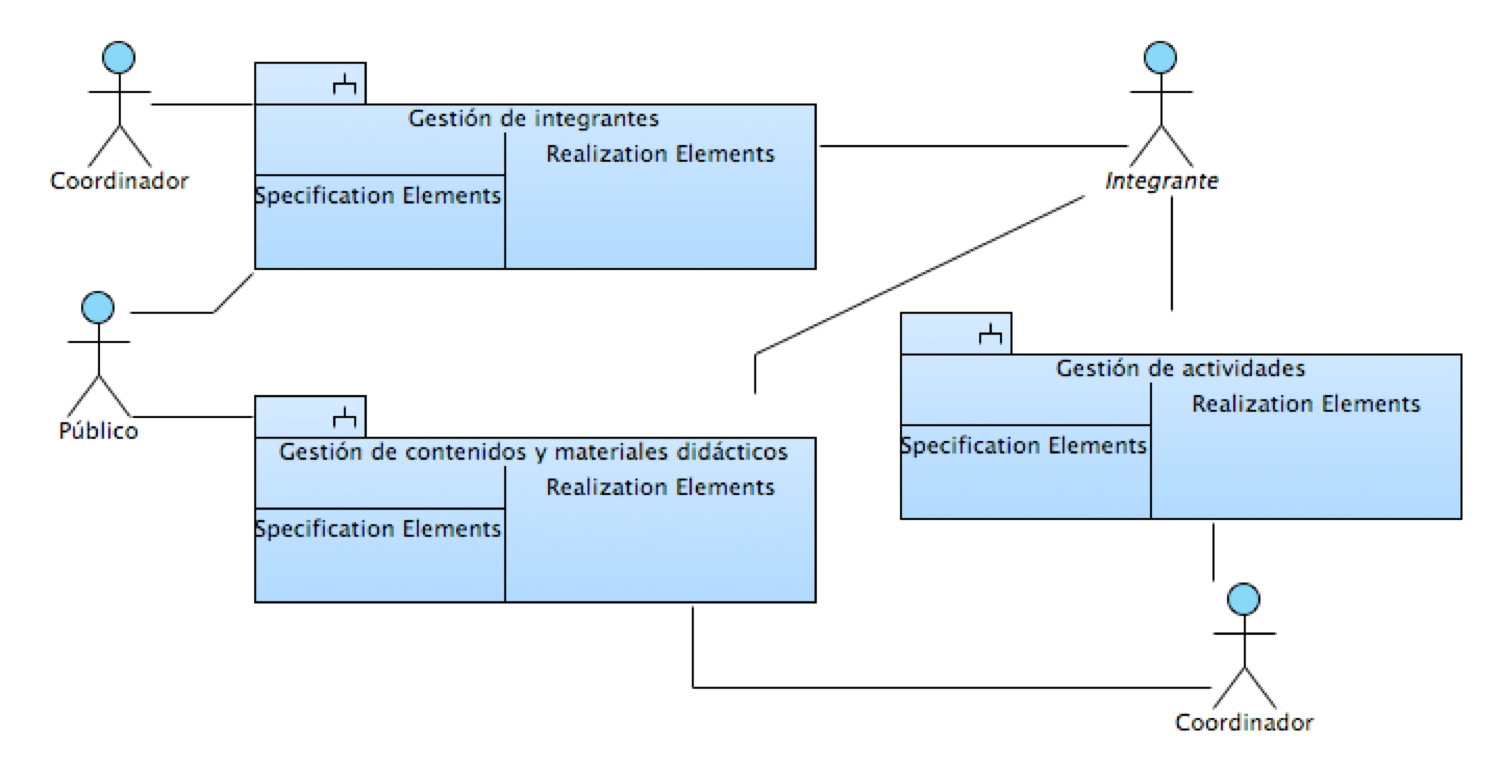
\includegraphics[width=.8\textwidth]{images/casosDeUso}}
		\caption{Diagrama de casos de uso del sistema.}
		\label{fig:casosDeUso}
	\end{center}
\end{figure}

\begin{figure}[htbp]
	\begin{center}
		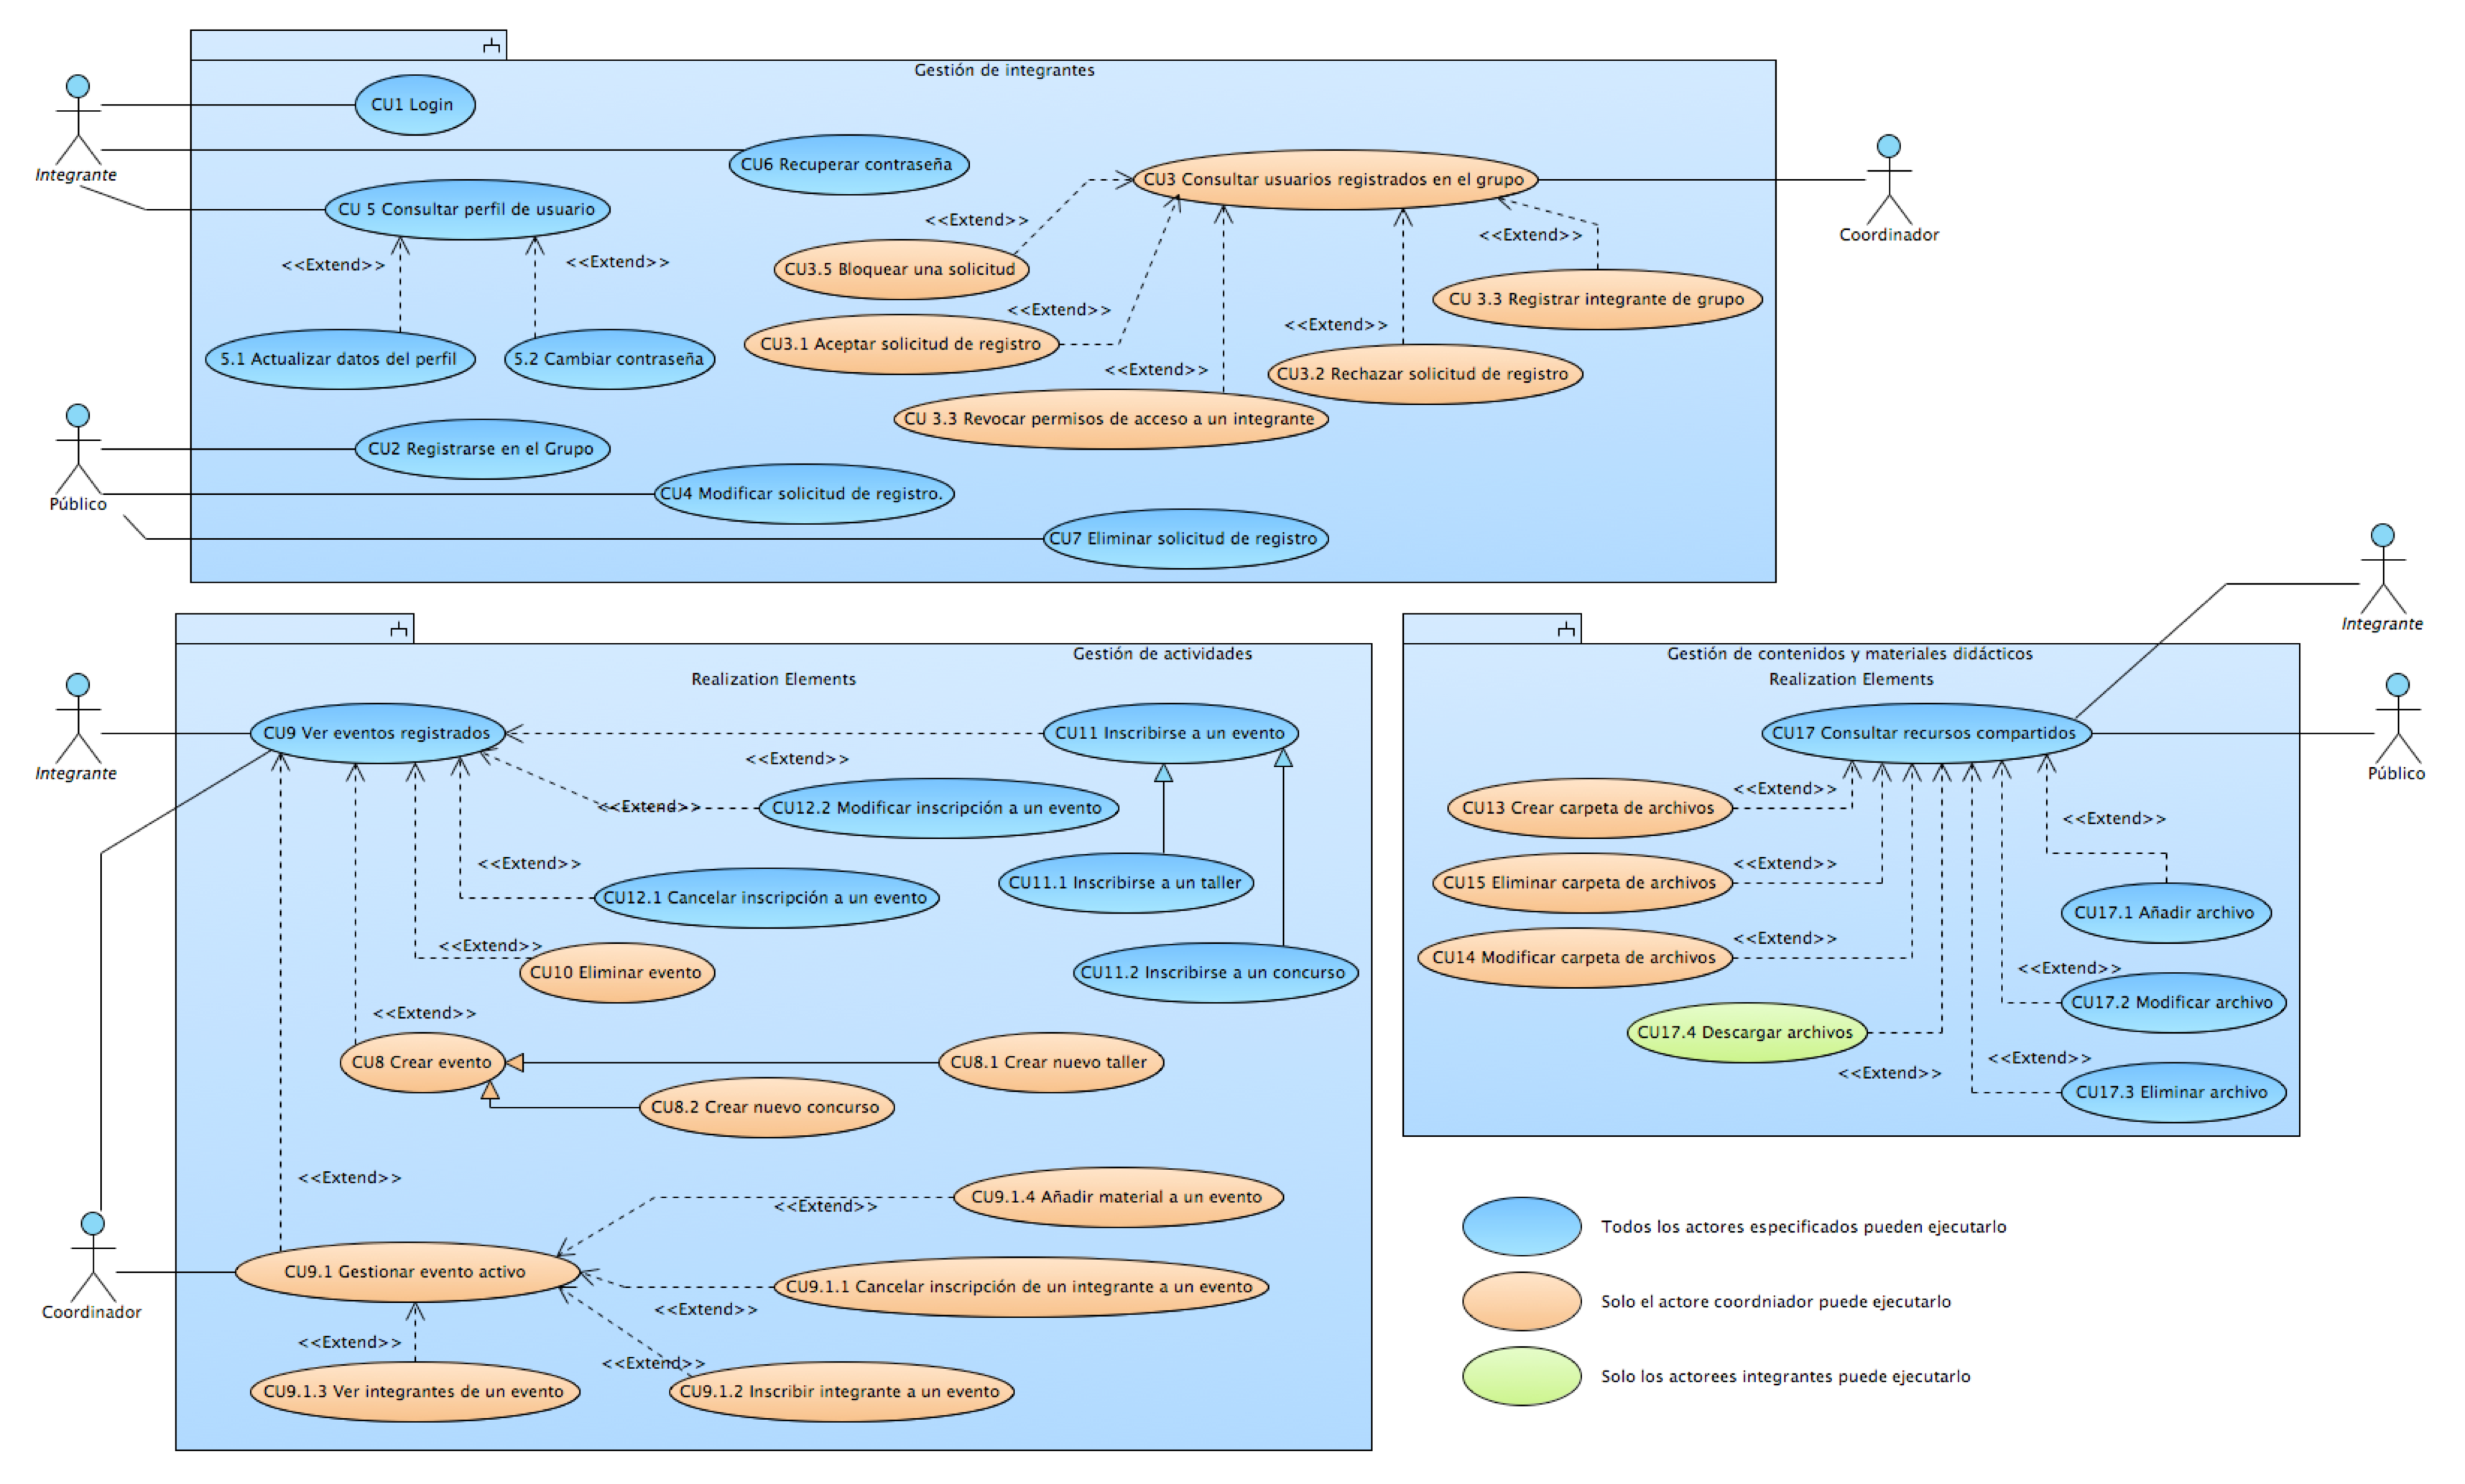
\includegraphics[angle=90, width=.7\textwidth]{images/casosDeUsoDetalle}
		\caption{Diagrama detallado del sistema.}
		\label{fig:casosDeUsoDetalle}
	\end{center}
\end{figure}

%---------------------------------------------------------

A continuación se detallan los casos de uso.

%---------------------------------------------------------
% CASOS DE USO

%% \IUref{IUAdmPS}{Administrar Planta de Selección}
% \IUref{IUModPS}{Modificar Planta de Selección}
% \IUref{IUEliPS}{Eliminar Planta de Selección}

% 


% Copie este bloque por cada caso de uso:
%-------------------------------------- COMIENZA descripción del caso de uso.

%\begin{UseCase}[archivo de imágen]{UCX}{Nombre del Caso de uso}{
%--------------------------------------
	\begin{UseCase}{CU17}{Inscribir a Seminario}{
		Ayudar a que los Estudiantes que están por terminar la carrera se puedan inscribir en un Seminario de titulación.
	}
		\UCitem{Versión}{\color{Gray}0.1}
		\UCitem{Autor}{\color{Gray}David Ortega Pacheco}
		\UCitem{Supervisa}{\color{Gray}Ulises Vélez Saldaña.}
		\UCitem{Actor}{\hyperlink{Alumno}{Alumno}}
		\UCitem{Propósito}{Que el Estudiante se pueda inscribir a un seminario de titulación.}
		\UCitem{Entradas}{Número de boleta, Contraseña y Seminario.}
		\UCitem{Origen}{Teclado}
		\UCitem{Salidas}{Seminarios registrados, horario actual del Estudiante, desglose del monto a pagar por la inscripción, recibo de pago y comprobante de inscripción.}
		\UCitem{Destino}{Pantalla e impresora para recibo de pago y comprobante de inscripción}
		\UCitem{Precondiciones}{El estudiante debe estar registrado en la universidad.}
		\UCitem{Postcondiciones}{El estudiante quedará inscrito en el Seminario seleccionado si es elegible y hay cupo en el Seminario en cuestión.}
		\UCitem{Errores}{}
		\UCitem{Tipo}{Caso de uso primario}
		\UCitem{Observaciones}{}
	\end{UseCase}
%--------------------------------------
	\begin{UCtrayectoria}{Principal}
		\UCpaso[\UCactor] Introduce su Número de Boleta y Contraseña en el sistema vía la  \IUref{IU23}{Pantalla de Control de Acceso}\label{CU17Login}.
		\UCpaso[\UCactor] Confirma la operación presionando el botón \IUbutton{Entrar}.
		\UCpaso Verifica que el Estudiante sea elegible para inscribirse al Seminario con base en la regla \BRref{BR129}{Determinar si un Estudiante puede inscribir Seminario.} \Trayref{A}.
		\UCpaso Despliega la \IUref{IU32}{Pantalla de Selección de Seminario} con la lista de Seminarios Disponibles.
		\UCpaso[\UCactor] Selecciona el Seminario en el que desea inscribirse \Trayref{B}\label{CU17SeleccionarSeminario}.
		\UCpaso Verifica que el Estudiante sea elegible para inscribirse al seminario seleccionado con base en la regla \BRref{BR130}{Determinar si un Estudiante puede inscribirse en un Seminario} \Trayref{C}.
		\UCpaso Verifica que el horario del Seminario concuerde con el horario del Estudiante con base en la regla \BRref{BR143}{Validar el horario del estudiante} \Trayref{D}.
		\UCpaso Calcula el costo del Seminario basado en el costo publicado en el catálogo de cursos, los costos aplicables al alumno y los impuestos aplicables, con base en las reglas \BRref{BR180}{Calcular costos del Estudiante} y \BRref{BR45}{Calcular impuestos por seminario}.
		\UCpaso Despliega el desglose de costos en la \IUref{IU33}{Pantalla Mostrar costos por seminario}.
		\UCpaso Pide al Estudiante que confirme la inscripción alSeminario.
		\UCpaso[\UCactor] Confirma la inscripción al Seminario.
		\UCpaso Inscribe al Estudiante en el Seminario seleccionado.
		\UCpaso Informa que la inscripción se realizó exitosamente vía la \IUref{UI88}{Pantalla de resumen de inscripción al Seminario}. 
		\UCpaso Imprime el recibo de pago con base en la regla \BRref{BR100}{Recibo del Estudiante por inscripción a Seminario.}.
		\UCpaso Pregunta al estudiante si desea imprimir un comprobante de la inscripción.
		\UCpaso[\UCactor] Indica que desea imprimir el comprobante de la inscripción.
		\UCpaso Imprime el comprobante de la inscripción \IUref{IU189}{Reporte de inscripción a Seminario}.		
	\end{UCtrayectoria}

%--------------------------------------		
		\begin{UCtrayectoriaA}{A}{El Estudiante no puede inscribir un Seminario}
			\UCpaso Muestra el Mensaje {\bf MSG1-}``El Estudiante [{\em Número de Boleta}] aun no puede inscribirse al seminario.''.
			\UCpaso[\UCactor] Oprime el botón \IUbutton{Aceptar}.
			\UCpaso[] Termina el caso de uso.
		\end{UCtrayectoriaA}
		
%--------------------------------------
		\begin{UCtrayectoriaA}{B}{El Estudiante abandona la operación}
			\UCpaso El Estudiante revisa la lista de Seminarios y no encuentra el Seminario que desea.
			\UCpaso[\UCactor] Oprime el botón \IUbutton{Salir}.
			\UCpaso Cierra la sesión del usuario.
			\UCpaso Continua en el paso \ref{CU17Login} del \UCref{CU17}.
		\end{UCtrayectoriaA}

%--------------------------------------
		\begin{UCtrayectoriaA}{C}{El estudiante no cumple con los prerrequicitos}
			\UCpaso Muestra el Mensaje {\bf MSG2-}``El Estudiante [{\em Número de Boleta}] no cumple con los requisitos para inscribirse al Seminario [{\em Nombre del Seminario seleccionado}].''.
			\UCpaso Muestra los requisitos que el Seminario seleccionado solicita.
			\UCpaso Continúa en el paso \ref{CU17SeleccionarSeminario} del \UCref{CU17}.
		\end{UCtrayectoriaA}

%--------------------------------------
		\begin{UCtrayectoriaA}{D}{El horario es incompatible.}
			\UCpaso Muestra el Mensaje {\bf MSG3-}``El horario del [{\em Nombre del Seminario seleccionado}] no es compatible con el horario del curso [{\em Nombre de la materia y grupo del curso con el que choca el horario}].''.
			\UCpaso Continúa en el paso \ref{CU17SeleccionarSeminario} del \UCref{CU17}.
		\end{UCtrayectoriaA}

%--------------------------------------
		
		
		
%-------------------------------------- TERMINA descripción del caso de uso.
% \IUref{IUAdmPS}{Administrar Planta de Selección}
% \IUref{IUModPS}{Modificar Planta de Selección}
% \IUref{IUEliPS}{Eliminar Planta de Selección}

% Copie este bloque por cada caso de uso:
%-------------------------------------- COMIENZA descripción del caso de uso.

%\begin{UseCase}[archivo de imágen]{UCX}{Nombre del Caso de uso}{
%--------------------------------------
\begin{UseCase}{CU01}{Alta a un nuevo empleado}{
}   
    \UCitem{Id}{MDS-SIGRES-CU-01}
    \UCitem{Descripción}{El Gerente de Recursos Humanos y/o un Agente de Recursos Humanos requiere dar de alta en el sistema a un empleado recién contratado.}
    \UCitem{Propósito}{Ingresar los datos de un nuevo empleado para que Gerentes de los distintos departamentos sean capaces de conocer la información persona de su plantilla de trabajo.}
    \UCitem{Precondiciones}{El Gerente de Recursos Humanos y/o Agente de Recursos Humanos debe estar registrado en el sistema.}
    \UCitem{Postcondiciones}{El nuevo empleado podrá acceder al sistema con su identificador correspondiente. Los datos del nuevo empleado podrán ser visualizados y modificados.}
    \UCitem{Entradas}{Datos personales del empleado como: nombre completo, dirección, teléfono fijo (opcional), teléfono celular, dirección de correo electrónico, situación, departamento, tipo de empleado.}
    \UCitem{Origen}{Teclado}
    \UCitem{Salidas}{Mensaje de Notificación, visualización de datos del empleado.}
    \UCitem{Destino}{Base de datos.}
    \UCitem{Errores}{El Gerente de Recursos Humanos y/o Agente de Recursos Humanos ingresa datos en un formato distinto al específicados u omite uno de los datos obligatorios.}
    \UCitem{Prioridad}{Alta}
    \UCitem{Volatilidad}{Alta}
    \UCitem{Madurez}{Media}
    \UCitem{Versión}{\color{Gray}0.3}
    \UCitem{Estatus}{En desarrollo}
    \UCitem{Autor}{\color{Gray}Daniela Rodríguez García}
    \UCitem{Revisor}{\color{Gray}Alejandro Bravo Torres}
    \UCitem{Fuentes}{RU57, RU61}
\end{UseCase}
%--------------------------------------
\begin{UCtrayectoria}{Principal}
\UCpaso[\UCactor] Introduce su identificador de Usuario y Contraseña en el sistema vía la  \IUref{IU23}{Pantalla de Control de Acceso}\label{CU17Login}.

\UCpaso[\UCactor] Confirma la operación presionando el botón \IUbutton{Entrar}.

\UCpaso Visualiza la \IUref{IU09}{Administración de Recursos Humanos} Administración de Recursos Humanos
\UCpaso[\UCactor] Ingresa al Menu de Empleados.

\UCpaso[\UCactor] Oprime la opción \IUbutton{Alta de nuevos empleados}.

\UCpaso[\UCactor] Ingresa los datos .

\UCpaso Se despliega la \IUref{IU10}{Confirmación de Alta de Nuevo Empleado} Confirmación de Alta de Nuevo Empleado.

\UCpaso El sistema almacena los datos del nuevo empleado.

\UCpaso [\UCactor] Regresa a la \IUref{IU09}{Administración de Recursos Humanos} Administración de Recursos Humanos.


\end{UCtrayectoria}

%--------------------------------------		
\begin{UCtrayectoriaA}{A}{El Gerente de Recursos Humanos y/o Agente de Recursos Humanos aborta el ingreso del nuevo empleado.}
\UCpaso [\UCactor] Presiona \IUbutton{
Cancelar} y se despliega la \IUref{IU11}{Confirmación de cancelación de Alta de Nuevo Empleado}
\UCpaso El sistema regresa a la Pantalla de Administración de Recursos Humanos. No se almacena ningún dato.
\end{UCtrayectoriaA}

\begin{UCtrayectoriaA}{B}{El Gerente de Recursos Humanos y/o Agente de Recursos Humanos no ingresa un dato que es obligatorio}
\UCpaso [\UCactor] Omite un dato obligatorio al dar de alta al nuevo empleado.
\UCpaso Se despliega la \IUref{IU12}{Error de inserción de datos}
\end{UCtrayectoriaA}

%--------------------------------------
% Puntos de extensión


%-------------------------------------- TERMINA descripción del caso de uso.

% \IUref{IUAdmPS}{Administrar Planta de Selección}
% \IUref{IUModPS}{Modificar Planta de Selección}
% \IUref{IUEliPS}{Eliminar Planta de Selección}

% 


% Copie este bloque por cada caso de uso:
%-------------------------------------- COMIENZA descripción del caso de uso.

%\begin{UseCase}[archivo de imágen]{UCX}{Nombre del Caso de uso}{
%--------------------------------------
\begin{UseCase}{CU03}{Visualización de los datos del empleado}{ }
    \UCitem{Versión}{\color{Gray}0.1}
    \UCitem{Autor}{\color{Gray}Daniela Rodríguez García}
    \UCitem{Supervisa}{\color{Gray}Joel Santillán Yáñez}
    \UCitem{Actor}{\hyperlink{Gerente de Recursos Humanos}{Gerente de Recursos Humanos, Agente de Recursos Humanos}}
    \UCitem{Propósito}{El Gerente de Recursos Humanos y/o Agente de Recursos Humanos visualice correctamente los datos asociados a un empleado.}
    \UCitem{Entradas}{Identificador de empleado.}
    \UCitem{Origen}{Teclado}
    \UCitem{Salidas}{Mensaje de Notificación, visualización de datos del empleado.}
    \UCitem{Destino}{Pantalla.}
    \UCitem{Precondiciones}{El Gerente de Recursos Humanos y/o Agente de Recursos Humanos y el empleado a visualizar sus datos deben estar registrado en el sistema.}
    \UCitem{Postcondiciones}{El Gerente de Recursos Humanos y/o Agente de Recursos Humanos podrá visualizar los datos de un empleado específico.}
    \UCitem{Errores}{El Gerente de Recursos Humanos y/o Agente de Recursos Humanos ingresa un identificador erróneo.}
    \UCitem{Tipo}{Caso de uso primario}
    \UCitem{Observaciones}{}
\end{UseCase}
%--------------------------------------
\begin{UCtrayectoria}{Principal}
\UCpaso[\UCactor] Introduce su identificador de Usuario y Contraseña en el sistema vía la  \IUref{IU23}{Pantalla de Control de Acceso}\label{CU17Login}.

\UCpaso[\UCactor] Confirma la operación presionando el botón \IUbutton{Entrar}.

\UCpaso Visualiza la \IUref{IU09}{Administración de Recursos Humanos} Administración de Recursos Humanos

\UCpaso[\UCactor] Ingresa al Menu de Empleados.

\UCpaso[\UCactor] Oprime la opción \IUbutton{Consulta de empleados}.

\UCpaso[\UCactor] Ingresa el identificador correspondiente del empleado a consultar.

\UCpaso Se despliega la \IUref{IU13}{Información del empleado} Información del empleado..

\UCpaso [\UCactor] Regresa a la \IUref{IU09}{Administración de Recursos Humanos} Administración de Recursos Humanos.


\end{UCtrayectoria}

%--------------------------------------		
\begin{UCtrayectoriaA}{A}{El Gerente de Recursos Humanos y/o Agente de Recursos Humanos ingresa un identificador de empleado erróneo.}
\UCpaso [\UCactor] Ingresa un identificador de empleado erróneo.
\UCpaso Se despliega la \IUref{IU14}{Identificador de empleado erróneo} Identificador de empleado erróneo.
\end{UCtrayectoriaA}

%--------------------------------------
% Puntos de extensión


%-------------------------------------- TERMINA descripción del caso de uso.
% \IUref{IUAdmPS}{Administrar Planta de Selección}
% \IUref{IUModPS}{Modificar Planta de Selección}
% \IUref{IUEliPS}{Eliminar Planta de Selección}

% 


% Copie este bloque por cada caso de uso:
%-------------------------------------- COMIENZA descripción del caso de uso.

%\begin{UseCase}[archivo de imágen]{UCX}{Nombre del Caso de uso}{
%--------------------------------------
\begin{UseCase}{CU14}{Eliminar Agente de Ventas}{
	El Gerente de Ventas elimina de forma logia la información de un Agente de Ventas.
}
    \UCitem{Versión}{\color{Gray}0.1}
    \UCitem{Autor}{\color{Gray}Alejandro Bravo Torres}
    \UCitem{Supervisa}{\color{Gray}Joel Santillán Yáñez}
    \UCitem{Actor}{\hyperlink{Gerente de Ventas}{Gerente de Ventas}}
    \UCitem{Propósito}{Que el gerente de Ventas pueda eliminar de forma lógicala información de un Cliente.}
    \UCitem{Entradas}{Número de Cliente.}
    \UCitem{Origen}{Teclado}
    \UCitem{Salidas}{Mensaje de Notificación, Cambio del Estado del Cliente.}
    \UCitem{Destino}{Pantalla para mensaje de coprobación.}
    \UCitem{Precondiciones}{El Gerente de Ventas y el Cliente deben estar registrados en el Sistema.}
    \UCitem{Postcondiciones}{El Agente de Ventas quedará inactivo de operación, es decir no podrá tener acceso ni participación en operaciones del sistema..}
    \UCitem{Errores}{}
    \UCitem{Tipo}{Caso de uso primario}
    \UCitem{Observaciones}{}
\end{UseCase}
%--------------------------------------
\begin{UCtrayectoria}{Principal}
\UCpaso[\UCactor] Introduce su Número de Usuario y Contraseña en el sistema vía la  \IUref{IU23}{Pantalla de Control de Acceso}\label{CU17Login}.

\UCpaso[\UCactor] Confirma la operación presionando el botón \IUbutton{Entrar}.

\UCpaso[\UCactor] Ingresa al Menu de Clientes.

\UCpaso[\UCactor] Ingresa el número de Cliente en el campo de Búsqueda.

\UCpaso Realiza la busqueda y devuelve el resultado.

\UCpaso[\UCactor] Verifia que el Cliente sea seleccionable para eliminacion

\UCpaso[\UCactor] Selecciona la Opción de \IUbutton{Eliminar} del registro en la tabla de Clientes.

\UCpaso Despliega la \IUref{IU32}{Pantalla de Confirmación de Eliminación de Ciente}. Pantalla de Confiracion de Eliminación de Cliente.  \Trayref{A}. 

\UCpaso El sistema realiza un borrado Lógico, cambio de status, al Cliente.

\UCpaso Regresa a la Pantalla principal de Administración de Clientes.


\end{UCtrayectoria}

%--------------------------------------		
\begin{UCtrayectoriaA}{A}{El Gerente de Ventas Cancela la Eliminación del Cliente.}
\UCpaso El sistema regresa al aPantalla Principal de Administración de Clientes. No se modifica ningún Cliente. 
\end{UCtrayectoriaA}
%--------------------------------------
% Puntos de extensión


%-------------------------------------- TERMINA descripción del caso de uso.
% \IUref{IUAdmPS}{Administrar Planta de Selección}
% \IUref{IUModPS}{Modificar Planta de Selección}
% \IUref{IUEliPS}{Eliminar Planta de Selección}

% 


% Copie este bloque por cada caso de uso:
%-------------------------------------- COMIENZA descripción del caso de uso.

%\begin{UseCase}[archivo de imágen]{UCX}{Nombre del Caso de uso}{
%--------------------------------------
	\begin{UseCase}{CU15}{Eliminar Agente de Ventas}{
		El Gerente de Ventas elimina de forma logia la información de un Agente de Ventas.
	}
		\UCitem{Versión}{\color{Gray}0.1}
		\UCitem{Autor}{\color{Gray}Alejandro Bravo Torres}
		\UCitem{Supervisa}{\color{Gray}Daniela Rodríguez García }
		\UCitem{Actor}{\hyperlink{Gerente de Ventas}{Gerente de Ventas}}
		\UCitem{Propósito}{Que el gerente de Ventas pueda eliminar la información de un Agente de Ventas.}
		\UCitem{Entradas}{Número de Empleado.}
		\UCitem{Origen}{Teclado}
		\UCitem{Salidas}{Mensaje de Notificación, Cambio del Estado del Agente de Ventas..}
		\UCitem{Destino}{Pantalla para mensaje de coprobación.}
		\UCitem{Precondiciones}{El Gerente de Ventas y el Agente de Ventas deben estar registrados en el Sistema.}
		\UCitem{Postcondiciones}{El Agente de Ventas quedará inactivo de operación, es decir no podrá tener acceso ni participación en operaciones del sistema..}
		\UCitem{Errores}{}
		\UCitem{Tipo}{Caso de uso primario}
		\UCitem{Observaciones}{}
	\end{UseCase}
%--------------------------------------
	\begin{UCtrayectoria}{Principal}
		\UCpaso[\UCactor] Introduce su Número de Usuario y Contraseña en el sistema vía la  \IUref{IU23}{Pantalla de Control de Acceso}\label{CU17Login}.
		
		\UCpaso[\UCactor] Confirma la operación presionando el botón \IUbutton{Entrar}.
		
		\UCpaso[\UCactor] Ingresa al Menu de Administración de Agentes
		
		\UCpaso Verifica que el Agente de Ventas sea elegible para Eliminar.
		
		\UCpaso[\UCactor] Selecciona la Opción de \IUbutton{Eliminar} del registro en la tabla de Agentes.
		
		\UCpaso Despliega la \IUref{IU32}{Pantalla de Confirmación de Eliminación de Empleado}. Pantalla de Confiracion de Eliminación de Empleado.  \Trayref{A}. 
		
		\UCpaso El sistema realiza un borrado Lógico, cambio de status, al Agente de ventas.
		
		\UCpaso Regresa a la Pantalla principal de Administración de Agentes.
		
		
	\end{UCtrayectoria}

%--------------------------------------		
		\begin{UCtrayectoriaA}{A}{El Gerente de Ventas Cancela la Eliminación del Agente.}
			\UCpaso El sistema regresa al aPantalla Principal de Administración de Empleados. No se modifica ningún Agente de Ventas. 
		\end{UCtrayectoriaA}
%--------------------------------------
% Puntos de extensión
	
		
%-------------------------------------- TERMINA descripción del caso de uso.




